% Author: Sarah Lang
% Website: latex-ninja.com
% License: Creative Commons CC BY 4.0
% Edited on 14/09/2022 for use on app.craftadoc.com


\documentclass[11pt]{article}


\usepackage{one-row-acad-cv}

%<{type: "group", description: "Personal information"}
\newcommand{\yourfirstname}
{JACK} %<{type: "text", description: "First name", id: "firstName"}>
\newcommand{\yourlastname}
{SPARROW} %<{type: "text", description: "Last name", id: "lastName"}>
\setNameToFancyFooter{\yourfirstname{ }\yourlastname}



\colorlet{cvthemecolour}{black}
%------------------------------------------------------------
% put in another colour instead of cyan to change the colour
%------------------------------------------------------------
\colorlet{cvcolour}{black!20}
    \begin{document}
    \pagestyle{pagenumbering}
    % -----------------------------------------------------------
    % The PHOTO and INFO BOX
    % -----------------------------------------------------------
    \begin{minipage}[t]{0.22\textwidth}
        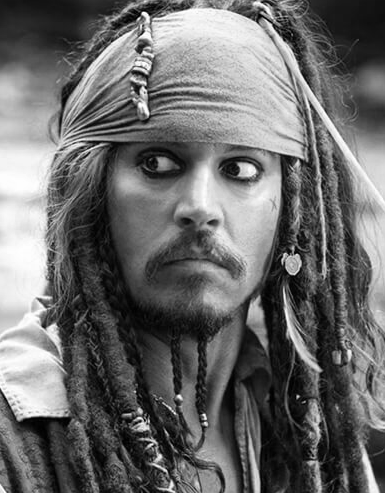
\includegraphics[valign=t,width=\textwidth]{jack-bw.png} %<{type: "crop", description: "Profile picture", aspect: 0.75, id: "profilePicture"}>
    \end{minipage}\hspace{1em}\hfill
    \begin{minipage}[t]{0.7\textwidth}
        
        \vspace{2em}
        \flushright
        \begin{tabular}[t]{r|c}
            {0043/800 010 100} %<{type: "phonenumber", description: "Phone number", id: "phoneNumber"}>
            & \faPhone  \\
            {Address Line}& \faHome \\ %<{type: "text", description: "Your address (optional)", deleteOnEmpty: true, id: "address"}>
            {Town, Country} %<{type: "text", description: "Your location (city, country)", id: "location"}>
            & \faMapMarker \\
            \texttt{jack@sparrow.com} & %<{type: "email", description: "Email address", id: "emailAddress"}>
            \faAt \\ 
            \texttt{www.sparrow.com}& \faLaptop %<{type: "text", description: "Website / homepage (optional)", deleteOnEmpty: true, id: "emailAddress"}>
            
        \end{tabular}
    \end{minipage}
    
    \vspace{1em}
%>
% -----------------------------------------------------------
% the NAME
% -----------------------------------------------------------
\headerrule{cvcolour}{1.3em} 
\nametag{\yourfirstname} 
{ }
{\yourlastname} 
\headerrule{cvcolour}{1.3em} % 0.45cm


% -----------------------------------------------------------
%<{type: "group", description: "About me"}
    \section{About me} %<{description: "Custom title (optional)", type: "text"}>
    %<{description: "Introduce yourself", "type": "textblock"}
    {Donec et nisl id sapien blandit mattis. Aenean dictum odio sit amet risus. Morbi purus. Nulla a est sit amet
    purus venenatis iaculis. Vivamus viverra purus vel magna. Donec in justo sed odio malesuada dapibus. Nunc
    ultrices aliquam nunc. Vivamus facilisis pellentesque velit. Nulla nunc velit, vulputate dapibus, vulputate id,
    mattis ac, justo. Nam mattis elit dapibus purus. Quisque enim risus, congue non, elementum ut, mattis quis,
    sem. Quisque elit.}
    %>
%>

\vspace{2em}

%<{description: "Certificates, degrees (or other topics you choose)", type: "list", deleteOnEmpty: true}
    %<{description: "", type: "group"}
        \subsection{CERTIFICATES} %<{description: "Section title", type: "text"}>
        \begin{tabular}{r p{0.8\textwidth}}
        %<{description: "List your items", type: "list"}
            %<{"description": "", "type": "group"}
                {2017--2019} %<{description: "Period (eg 2017--2019)", type: "text", maxLength: 10}>
                & \textbf{Pirate Trainer} \newline %<{description: "Achievement/job title", type: "text"}>
                { Lorem Ipsum Dolor Sit Amet. } \\ %<{description: "Achievement/job description", type: "text"}>
            %>
            2016--2017 & \textbf{Captain Training} \newline
                { Lorem Ipsum Dolor Sit Amet. Lorem Ipsum Dolor Sit Amet. \newline Lorem Ipsum Dolor Sit Amet. }
        %>
        \end{tabular}
        
        \cvrule{black}{2pt}
    
    %>
    \subsection{DEGREES}
    \begin{tabular}{r p{0.8\textwidth}}
        \cvdegree{1710}{Captain}{Certified}{Tortuga Uni \color{cvcolour}}{}{disney.png} \\
        \cvdegree{1715}{Bucaneering}{M.A.}{London \color{cvcolour}}{test}{medal.jpeg} \\
        \cvdegree{1720}{Bucaneering}{B.A.}{London \color{cvcolour}}{}{medal.jpeg}
    \end{tabular}
    
    \cvrule{black}{2pt}

%>

%<{description: "Work experience, internships, teaching experience (or other topics you choose)", "type": "list", deleteOnEmpty: true}
%<{description: "", type: "group"}
\subsection{WORK EXPERIENCE}%<{description: "Section title", type: "text"}>
\begin{tabular}{r| p{0.8\textwidth}}
    %<{description: "Section items", type: "list"}
    %<{"description": "", "type": "group"}
        \cvevent{2018--2021}%<{description: "Period (e.g. 2011--2012)", type: "text", maxLength: 10}>
        {Captain of the Black Pearl}%<{description: "Item title", type: "text"}>
        {Lead}%<{description: "Role", type: "text"}>
        {East Indies}%<{description: "Description", type: "text"}>
        \\
    %>
        \cvevent{2019}{Freelance Pirate}{Bucaneering}{Tortuga} \\
        \cvevent{2016--2017}{Captain of the Black Pearl}{Lead}{Tortuga}
    %>
\end{tabular}

\cvrule{black}{2pt}
%>


\subsection{INTERNSHIPS}
\begin{tabular}{r| p{0.8\textwidth}}
    \cvevent{2018--2021}{Captain of the Black Pearl}{Lead}{East Indies \color{cvcolour}}{Finally got the goddamn ship back.}{disney.png} \\
    \cvevent{2019}{Freelance Pirate}{Bucaneering}{Tortuga \color{cvcolour}}{This and that. The usual, aye?}{medal.jpeg} \\
    \cvevent{2016--2017}{Captain of the Black Pearl}{Lead}{Tortuga \color{cvcolour}}{Found a secret treasure, lost the ship.}{medal.jpeg}
\end{tabular}

\cvrule{black}{2pt}


\subsection{Teaching Experience}
\begin{tabular}{r| p{0.8\textwidth}}
    \cvevent{2018--2021}{Captain of the Black Pearl}{Lead}{East Indies \color{cvcolour}}{Finally got the goddamn ship back.}{disney.png} \\
    \cvevent{2019}{Freelance Pirate}{Bucaneering}{Tortuga \color{cvcolour}}{This and that. The usual, aye?}{medal.jpeg} \\
    \cvevent{2016--2017}{Captain of the Black Pearl}{Lead}{Tortuga \color{cvcolour}}{Found a secret treasure, lost the ship.}{medal.jpeg}
\end{tabular}

\cvrule{black}{2pt}

\subsection{Secondary Education}
\begin{tabular}{>{\itshape}r|l}
    2018 & Certificate \\
    1990 & Education Certificate \\
    2018 & Certificate Certificate\\
    1990 & Education
\end{tabular}

\cvrule{black}{2pt}

\subsection{Secondary Education}
\begin{tabular}{>{\itshape}r|l}
    2018 & Certificate \\
    1990 & Education Certificate \\
    2018 & Certificate Certificate\\
    1990 & Education
\end{tabular}

\vspace{1em}

\subsection{Tertiary Education}
\begin{tabular}{>{\itshape}r|l}
    2018 & Certificate \\
    1990 & Education Certificate \\
    2018 & Certificate Certificate\\
    1990 & Education
\end{tabular}

\cvrule{black}{2pt}

\subsection{FELLOWSHIPS \& PRIZES}
\begin{tabular}{r p{0.8\textwidth}}
2018--2020 & Personal Assistant of Captain Barbossa \\
2019 & Best Pirate Ever \\
2018--2020 & Personal Assistant of Captain Barbossa \\
2019 & Best Pirate Ever
\end{tabular}


\cvrule{black}{2pt}


\subsection{GRANTS \& AWARDS}
\begin{tabular}{r p{0.8\textwidth}}
2018--2020 & Personal Assistant of Captain Barbossa \\
2019 & Best Pirate Ever \\
2018--2020 & Personal Assistant of Captain Barbossa \\
2019 & Best Pirate Ever
\end{tabular}

\cvrule{black}{2pt}

\subsection{SCIENCE COMMUNICATION}

Blog: ``Sparrow and the Birds'', \protect\url{https://sparrow.com/}.


\cvrule{black}{2pt}

\subsection{TRAININGS GIVEN}
\begin{tabular}{r| p{0.8\textwidth}}
        \cvevent{2019}{Cheating}{Bucaneering}{Royal Institution}{}{} \\
    \cvevent{2019}{Stealing}{Bucaneering}{Royal Institution}{}{} \\
     \cvevent{2018}{Be Your Best Pirate Self}{Bucaneering}{Royal Institution}{}{} \\
\end{tabular}

\cvrule{black}{2pt}

\subsection{SOCIETIES}
\begin{tabular}{>{\itshape}r|p{0.8\textwidth}}
ab 2019 & The Royal Society \\
ab 2018 & Pirates' Club \\
ab 2019 & The Royal Society \\
ab 2018 & Pirates' Club
\end{tabular}



\cvrule{black}{2pt}


\subsection{PUBLICATIONS}
\begin{tabular}{>{\bfseries}r >{}p{0.8\textwidth}}
    1729\hspace{-0.5em} & \emph{How I almost got killed by Lady Swan}, in: Barbossa (ed.): \emph{Proceedings of the Pirate's Conference}, Tortuga Printing Press. \\
    1720\hspace{-0.5em} & ``Privateering for Beginners'', in: \emph{The Pragmatic Pirate} (1/1720).\\
    1729\hspace{-0.5em} & \emph{How I almost got killed by Lady Swan}, in: Barbossa (ed.): \emph{Proceedings of the Pirate's Conference}, Tortuga Printing Press. \\
    1720\hspace{-0.5em} & ``Privateering for Beginners'', in: \emph{The Pragmatic Pirate} (1/1720).
\end{tabular}






\cvrule{black}{2pt}

\section*{Degrees}
\begin{tabular}{r p{0.8\textwidth}}
    \cvdegree{1710}{Captain}{Certified}{Tortuga Uni \color{cvcolour}}{}{disney.png} \\
    \cvdegree{1715}{Bucaneering}{M.A.}{London \color{cvcolour}}{test}{medal.jpeg} \\
    \cvdegree{1720}{Bucaneering}{B.A.}{London \color{cvcolour}}{}{medal.jpeg}
\end{tabular}

\cvrule{black}{2pt}
%>

\subsection{LANGUAGES}
%<{description: "Languages", type: "list", deleteOnEmpty: true}
    %<{description: "Your language", type: "text"}
    {English (mother tongue).}
    
    %>
    
    French (parler).

    Spanish A1.
%>

\end{document}